\subsection{Komponentenprinzipien}
\label{sec:Komponentenprinzipien}

Komponenten sind die kleinsten veröffentlichbaren Einheiten eines Systems. In Java können sie als \code{.jar} Dateien in das System mit eingebunden werden. Komponenten können aber auch programmatisch in einem System eingebracht werden. Eine Komponente besitzt die Fähigkeit unabhängig von anderen Komponenten entwickelt zu werden \citep[vgl.][96]{martin2018}.

Komponenten weisen die Eigenschaft der Kohäsion und der Kopplung auf. Dabei existiert die Köhasion innerhalb einer Komponente und die Kopplung zwischen verschiedenen Komponenten \citep[vgl.][131]{voorhees2020}.

%Note the contrast between coupling and cohesion—coupling exists between two modules while cohesion exists within one module \citep[vgl.][131]{voorhees2020}.

Im Folgenden werden Prinzipien der Komponentenkohäsion und der "=kopplung vorgestellt. Dabei wird bei der Komponentenkopplung auf zwei Metriken (\textit{positional stability} und \textit{abstractness} einer Komponente) eingegangen, anhand deren man die Kopplung einzelner Komponenten untereinander bemessen kann.

\subsubsection{Komponentenkohäsion}

Das Ausmaß, wie Module innerhalb einer Komponente zusammenhängen, nennt sich Kohäsion. Eine hohe Kohäsion ist ein Merkmal gut entworfener Komponenten in einem System. Wenn Komponenten für Module verantwortlich sind, die nicht miteinander zusammenhängen, wurde die Funktionalität schlecht verteilt \citep[vgl.][797]{gui2009}.

%Cohesion is the extent to which the functions performed by a subsystem are related. If a subcomponent is responsible for a number of unrelated functions then the functionality has been poorly distributed to subcomponents. Hence high cohesion is a characteristic of a well designed subcomponent \citep[vgl.][797]{gui2009}.

Eine hohe Kohäsion ist auch daran zu erkennen, dass eine Komponente mit einer einzigen Aufgabe schwer in weitere Komponenten aufzuteilen ist und dass sich einzelne Module aus der Komponente nicht trennen lassen. Eine Komponente hingegen, deren Aufgabenbereich zu weit gefasst ist und zu viele Abhängigkeiten aufweist, kann folgende Probleme aufweisen: Sie ist schwer zu verstehen, wiederzuverwenden, zu pflegen und ständigen Änderungen ausgesetzt \citep[vgl.][131]{voorhees2020}.

%Having a module with one basic purpose that is hard to split into separate units is called high cohesion or strong cohesion. A good design is one that exhibits highly cohesive modules. Having a module that contains many basic purposes (i.e., many responsibilities) is called low cohesion or weak cohesion. A bad design is one that exhibits low cohesive modules.
%A class with low cohesion does many unrelated things or does too much work. Such classes are undesirable; they suffer from the following problems:
%• Hard to comprehend
%• Hard to reuse
%• Hard to maintain
%• Delicate; constantly affected by change \citep[vgl.][131]{voorhees2020}.

Zum Zusammenfassen von Komponenten gibt \citeauth{martin2018} drei Prinzipien vor:
\begin{itemize}
\item \ac{REP}
\item \ac{CCP}
\item \ac{CRP}
\end{itemize}

Softwarekomponenten, die wiederverwendet werden sollen, müssen für das \ac{REP} erst einem Releaseprozess unterlaufen und eine Versionsnummer erhalten \citep[vgl.][104]{martin2018}. Das bedeutet gleichzeitig, dass Module nicht einfach zu einer Komponente zusammengeworfen werden, sondern einer übergreifenden Aufgabe dienen sollen \citep[vgl.][105]{martin2018}.

%The Reuse/Release Equivalence Principle (REP) is a principle that seems obvious, at least in hindsight. People who want to reuse software components cannot, and will not, do so unless those components are tracked through a release process and are given release numbers \citep[vgl.][104]{martin2018}.

%From a software design and architecture point of view, this principle means that the classes and modules that are formed into a component must belong to a cohesive group. The component cannot simply consist of a random hodgepodge of classes and modules; instead, there must be some overarching theme or purpose that those modules all share \citep[vgl.][105]{martin2018}.

Beim \ac{CCP} wird verlangt, Module, die zur selben Zeit und aus demselben Grund geändert werden, in eine Komponente zu fassen. Wenn Module diese Eigenschaft nicht aufweisen, sollten sie in verschiedene Komponenten gegliedert werden \citep[vgl.][105]{martin2018}.
 
%Gather into components those classes that change for the same reasons and at the same times. Separate into different components those classes that change at different times and for different reasons \citep[vgl.][105]{martin2018}. 

%MAYBE: For most applications, maintainability is more important than reusability. If the code in an application must change, you would rather that all of the changes occur in one component, rather than being distributed across many components. If changes are confined to a single component, then we need to redeploy only the one changed component. Other components that don’t depend on the changed component do not need to be revalidated or redeployed \citep[vgl.][106]{martin2018}.

Das \ac{CRP} besagt, dass gemeinsam genutzte Komponenten in eine Komponente übergehen sollen, sofern sie immer miteinander verwendet werden. So werden unnötige Abhängkeiten vermieden \citep[vgl.][107]{martin2018}.

%Don’t force users of a component to depend on things they don’t need. It states that classes and modules that tend to be reused together belong in the same component \citep[vgl.][107]{martin2018}. 

%Therefore the CRP tells us more about which classes shouldn’t be together than about which classes should be together. The CRP says that classes that are not tightly bound to each other should not be in the same component \citep[vgl.][108]{martin2018}.
 

\subsubsection{Komponentenkopplung}

Kopplung ist die Interaktion von Komponenten untereinander. Wenn die Kopplung zwischen Komponenten stärker ist, kann eine Änderung an einer Komponente auch Änderungen an den abhängigen nach sich ziehen. Eine lose Kopplung ist daher eine gewünschte Eigenschaft \citep[vgl.][797]{gui2009}.

%Coupling is the extent to which the various subcomponents interact. If  hey are highly interdependent then changes to one are likely to have  significant effects on the behavior of others. Hence loose coupling  between its subcomponents is a desirable characteristic of a component \citep[vgl.][797]{gui2009}.

Umso weniger Verbindungen zwischen Komponenten bestehen, desto weniger Aufwand entsteht in der Wartung, Reparatur oder im Test einer Komponente. Ein gutes Design weist daher eine geringe Kopplung auf. Eine starke Kopplung hingegen bedeutet: Änderungen von Abhängigkeiten müssen in lokale Komponenten eingepflegt werden, eine Komponente ist isoliert schwieriger zu verstehen und die Wiederverwendung wird durch benötigte Abhängigkeiten schwieriger \citep[vgl.][130]{voorhees2020}.

%The coupling definitions indicate that coupling describes the amount of connectedness between two or more modules. Thus, a design that has only one module cannot exhibit coupling. That is, coupling can only be described between distinct modules. Our intuition suggests having fewer connections between modules mean there is less to test, maintain, and fix. Having fewer connections between modules is called low coupling, loose coupling, or weak coupling. A good design is one that exhibits low coupling between its modules. In contrast, more connections between modules means there is more to test, maintain, and fix. Having more connections between modules is called high coupling, tight coupling, or strong coupling. A bad design is one that exhibits high coupling between its modules  \citep[vgl.][130]{voorhees2020}.

%A class with high (or strong) coupling relies on many other classes. Such classes may be undesirable; some suffer from the following problems:
%• Changes in related classes force local changes
%• Harder to understand in isolation
%• Harder to reuse because its use requires the additional presence of the classes on which it is dependent   \citep[vgl.][130]{voorhees2020}.


Um Komponenten miteinander zu verbinden, gibt \citeauth{martin2018} drei verschiedene Prinzipien vor:
\begin{itemize}
\item \ac{ADP}
\item \ac{SDP}
\item \ac{SAP}
\end{itemize}

Das \ac{ADP} besagt, dass keine zyklischen Abhängigkeiten zwischen Komponenten erlaubt werden und es sich um einen \ac{DAG} handeln soll. Bei einem \ac{DAG} kann von einer beliebigen Stelle einem Pfad gefolgt werden, ohne wieder am Ausgangspunkt anzugelagen \citep[vgl.][114]{martin2018}. 

In \refAbbns{fig:adp_false} ist dies nicht der Fall. Das Problem kann aber auf zwei Arten behoben werden. Zum einen kann eine dritte Komponente mit entsprechenden Schnittstellen gebildet werden und beide Komponenten zeigen auf diese  (\refAbb{fig:adp_okay}). Die andere Variante ist die Anwendung vom \ac{DIP}. Hierdurch wird eine Schnittstelle in eine Komponente aufgenommen, wodurch sich die Beziehung umdreht (\refAbb{fig:adp_okay_2}).

\begin{figure}
  \centering
  \includegraphics[height=1.2cm]{build/generated-uml/adp_false.png}
   \caption{Zyklische Abhängigkeit zwischen zwei Komponenten.}
   \label{fig:adp_false}
\end{figure}

\begin{figure}
  \centering
  \includegraphics[height=1.2cm]{build/generated-uml/adp_okay.png}
   \caption{Auflösung der zyklischen Abhängigkeit durch eine dritte Komponente.}
   \label{fig:adp_okay}
\end{figure}

\begin{figure}
  \centering
  \includegraphics[width=5cm]{build/generated-uml/adp_okay_2.png}
   \caption{Auflösung der zyklischen Abhängigkeit durch Anwendung von \ac{DIP}. Die Verbindung von \code{A} nach \code{B} wird aufgelöst und umgekehrt. Die Beziehung besteht nur noch logisch (gestrichelter Pfeil). }
   \label{fig:adp_okay_2}
\end{figure}


%Allow no cycles in the component dependency graph \citep[vgl.][112]{martin2018}.

%Regardless of which component you begin at, it is impossible to follow the dependency relationships and wind up back at that component. This structure has no cycles. It is a directed acyclic graph (DAG) \citep[vgl.][114]{martin2018}. 

%It is always possible to break a cycle of components and reinstate the dependency graph as a DAG. There are two primary mechanisms for doing so ... \citep[vgl.][117]{martin2018}.
 
Das \ac{SDP} besagt, dass eine Komponente nur auf eine anderen Komponente verweisen soll, wenn diese stabiler ist. Dabei misst sich die \textit{positional stability} (im Folgenden Instabilität) anhand der Formel
\begin{equation}
I = F_o / (F_i + F_o).
\end{equation}
$F_i$ sind dabei die eingehenden Abhängigkeiten der Komponente. Hier werden alle Module gezählt, die auf die Komponente zugreifen. $F_o$ sind alle ausgehenden Abhängigkeiten, bei denen die Module gezählt werden, die außerhalb verwendet werden. $I$ ist die Instabilität und nimmt einen Wert zwischen $0$ und $1$ an. Bei einem Wert von $1$ gilt die Komponente als instabil, da sie von keiner anderen Komponente verwendet wird, aber selbst sehr viele andere Komponenten verwendet. Bei $0$ besitzt eine Komponente keine Abhängigkeiten, aber wird von anderen verwendet \citep[vgl.][122]{martin2018}.
 
%Depend in the direction of stability. 

%• Fan-in: Incoming dependencies. This metric identifies the number of classes outside this component that depend on classes within the component.
%• Fan-out: Outgoing depenencies. This metric identifies the number of classes inside this component that depend on classes outside the component.
%• I: Instability: I = Fan-out , (Fan-in + Fan-out). This metric has the range [0, 1]. I = 0 indicates a maximally stable component. I = 1 indicates a maximally unstable component \citep[vgl.][122]{martin2018}
  
\ac{SAP} besagt, eine Komponente sollte so abstrakt wie stabil sein \citep[vgl.][126]{martin2018}. Dadurch verlaufen Abhängigkeiten in Richtung der Abstraktion, wodurch automatisch instabile Komponenten auf stabile Komponenten verweisen. 

Der Grad $A$ der \textit{abstractness} lässt sich über 
\begin{equation}
A = N_a/N_c
\end{equation}
berechnen. Dabei ist $N_a$ die Anzahl aller abstrakten Module, $N_c$ ist die Anzahl aller Module. $A$ liegt im Bereich zwischen $0$ und $1$. Eine Komponente mit dem Wert $0$ ist dabei komplett konkret, da keine Schnittstellen in der Komponente vorhanden sind. Bei einem Grad von $1$ gibt es keine Implementierungsdetails, sondern alle Module sind Schnittstellen \citep[vgl.][127]{martin2018}.

%A component should be as abstract as it is stable  \citep[vgl.][126]{martin2018}.

%• Nc: The number of classes in the component.
%• Na: The number of abstract classes and interfaces in the component.
%• A: Abstractness. A = Na , Nc.
%The A metric ranges from 0 to 1. A value of 0 implies that the component has no abstract classes at all. A value of 1 implies that the component contains nothing but abstract classes  \citep[vgl.][127]{martin2018}.

Wenn beide Werte zusammengenommen werden, kann eine Komponente auf einem Graph, wie in \refAbbns{fig:i_a_graph}, verortet werden. Die Komponenten befinden sich idealerweise auf oder in der Nähe der Hauptreihe (\textit{Main Sequence}). Komponenten in der \textit{Zone of Pain} und der \textit{Zone of Uselessness} sollten vermieden werden. Solche Komponenten lassen sich schwer aktualisieren \bzw erfüllen schlicht keinen Zweck und sind damit nutzlos \citep[vgl.][128\psqq]{martin2018}. Die Distanz $D$ zu Hauptreihe berechnet sich mit 
\begin{equation}
D = |A + I -1|
\end{equation}
\citep[vgl.][130]{martin2018}.

\begin{figure}
  \centering
  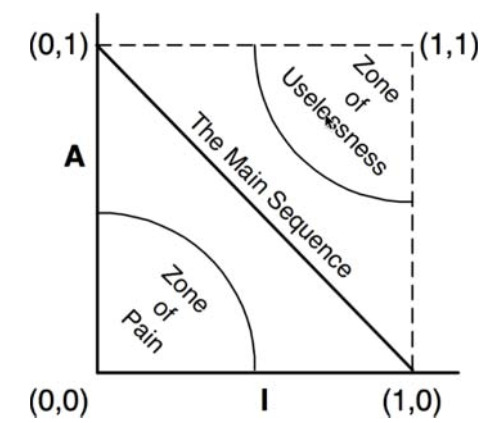
\includegraphics[width=7cm]{res/i_a_graph.jpg}
   \caption{Komponenten, deren Instabilität und Abstraktheit berechnet wurde, können in einem solchen Graphen verortet werden \citep[][128]{martin2018}.}
   \label{fig:i_a_graph}
\end{figure}


\citeauth{martin2018} trifft keine Aussage darüber, wann $D$ zu groß ist. Es wird nur gesagt, dass sich $D$ mit jeder Restrukturierung Null nähern soll.
